%\fancyhead[RO,LE]{\thepage}
%\fancyfoot{}
\chapter{\textbf{introduction}}

% With the rapid evolution of 5G and IoT recently, more and more applications, as exemplified by visual cloud computing, personalized firewalls, video encoders, and content caches, deep packet inspection, etc, have ca

% Due to the increasing growth of computational-intensive and delay

\section{Motivation}

Driven by the rapidly evolving modern communication technologies such as $5$G and beyond~\cite{6G_beyond}, 
the next generation of mobile applications such as virtual and augmented reality ~\cite{CloudTrans_2020}, face recognition~\cite{soyata2012cloud} and 3D interactive gaming~\cite{chen2019framework}, have become more and more prevalent and approachable in our daily life. 
The increasing development of these mobile applications result from recent growth in mobile device usage. According to the recent Cisco Annual Internet Report~\cite{forecast2019cisco}, the total number of global devices and connections are predicted to increase by  11 million, with a 2 million increase in mobile devices (Smartphones, Non-smartphones, Tablets, etc.). Figure~\ref{fig:device_growth} depicts the trend of the growth in global device usage. However, mobile devices often suffer from resource limits such as storage, computing capacity, battery lifetime and therefore cannot provide the aforementioned applications with the guaranteed low latency that they require.
\begin{figure}
	\centering
	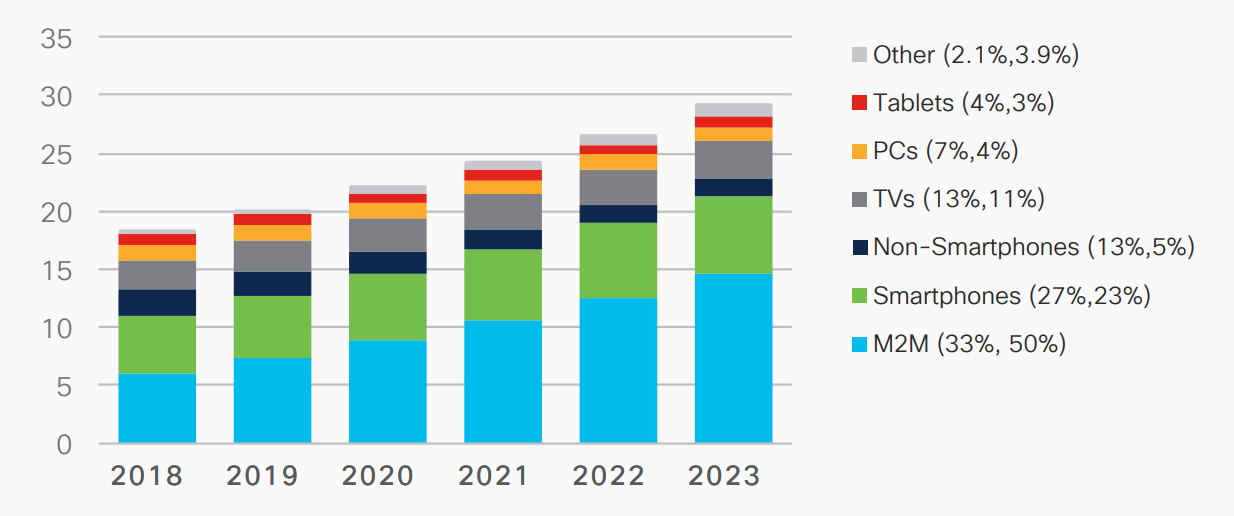
\includegraphics[width=.9\textwidth]{figs/devices growth.PNG}
		\vspace{\baselineskip}
	\caption{Global device and connection growth (billion)~\cite{forecast2019cisco}}
	\label{fig:device_growth}
\end{figure}


In order to address the computational limit of the local mobile devices, Mobile Edge Computing (MEC)~\cite{mec_wp} has recently been introduced as a promising architecture that has the potential to enable cellular networks to offer low latency to mobile applications. MEC equips cellular base stations (i.e., the edge) with computing and storage resources. Such an architecture allows mobile users to work with services deployed in their vicinity and avoid frequent communication with remote cloud services. However, the amount of available resources at the edge is scarce, and thus it is necessary to manage them efficiently to handle the ever-increasing user demands.

Recently, researchers \cite{sfcgeo, visualcomputing, yang2019delay, xu2020nfv} have proposed to apply NFV to MEC to provide more added-values, such as low cost and high efficiency. Network function virtualization (NFV) [4] has emerged as a networking-computing paradigm that enables efficient utilization of computing and networking resources by applying virtualization technologies to offer network services. In this paradigm, network services are implemented as software modules called virtual network functions (VNFs) that can be dynamically deployed, scaled, and chained together to offer a variety of services to users. In particular, the NFV paradigm is well suited to mobile environments where users freely roam at the edge of the network and dynamically change their point of attachment to the network. 
%A critical challenge of using NFV at the edge is the orchestration of service function chains (SFCs). Each SFC is an ordered sequence of VNFs that are chained together to process the user traffic in order to implement a specific network service. SFC orchestration is the problem of placement, routing, and migration of VNFs to minimize the user-perceived service latency with acceptable operational cost
In NFV, service demands are expressed in the form of Service Function Chains (SFCs). An SFC specifies a sequence of VNFs that user traffic has to pass through in order to attain the required service. 
%SFC is a common and flexible model to realize various services with different requirements, and it allows user to separate data processing in different computing units in MEC (\eg\ edge, cloud, local device) and therefore greatly boost processing time and reduce end-to-end latency while providing enhanced management. 
One of the main challenges of implementing SFCs in MEC is the placement of VNFs on the limited resources that are available at the edge, refer to as \textbf{SFC Orchestration}. User mobility further complicates the placement decisions, where due to user mobility, it may be possible to migrate an SFC or part of it closer to the new location of the user to reduce the communication delay, or continue to run the VNFs in their current locations to avoid service migration delays. Therefore, a trade-off between communication delay and migration delay is often considered when placing VNFs at the network edge.
%


\cat{Motiviating Example} An example of SFC orchestration in MEC can be illustrated in visual cloud computing for 3D light detection and ranging (LIDAR) \cite{visualcomputing}, which deal with different data processing stages such as: 1) acquisition; 2) preprocessing; 3) analysis; and 4) postprocessing. The LIDAR pipeline is outlined in figure 1. When scanning and modeling moving objects in 3D space, the processing stages are divided into two categories based on computational needs: (1) small instance processing: Camera metadata data processing, static background registration, and 3D rendering; (2) large instance processing: video camera pose computation, motion segmentation, and dynamic object positioning. In this example, we can consider each processing function as a service function in SFC orchestration, and a good strategy is to place small instance processing functions on the edge nodes that have limited computing resources but shorter access latency and place the large instance processing functions on the cloud that has sufficient capacity but longer access latency.
\begin{figure}
	\centering
	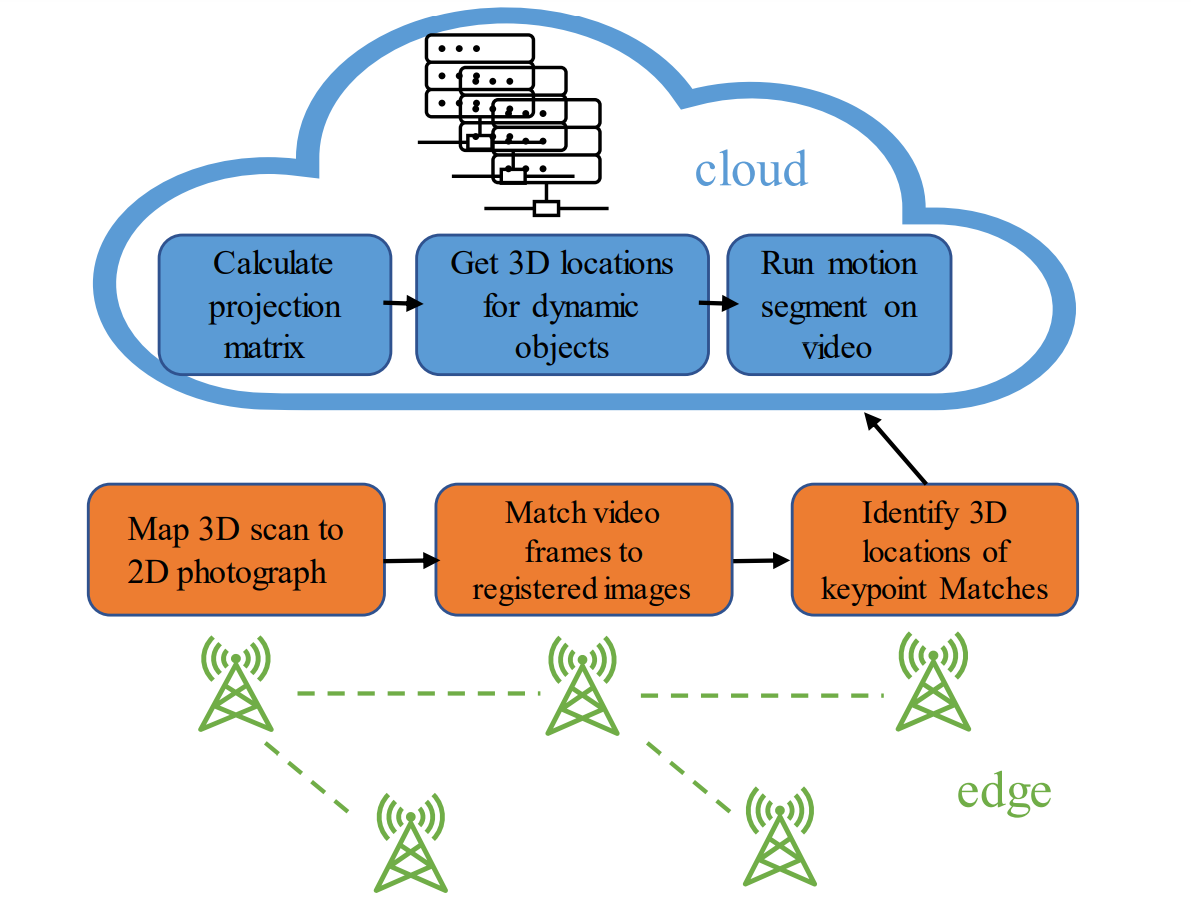
\includegraphics[width=0.9\textwidth]{figs/LIDAR.PNG}
		\vspace{\baselineskip}
	\caption{Example 1: visual cloud computing SFC for 3D light detection and ranging \cite{visualcomputing}}
	\label{fig:lidar}
\end{figure}

Another example of real-time SFC orchestration is shown in figure \ref{fig:geosfc}. This shows a geo-distributed latency sensitive SFC for the computer vision of a real-time object tracking pipeline\cite{sfcgeo}. The pre-processing and Human-Computer Interaction analysis functions are placed on the edge servers while the track function that involves
compute-intensive processing is placed on a cloud server. 
\begin{figure}
	\centering
	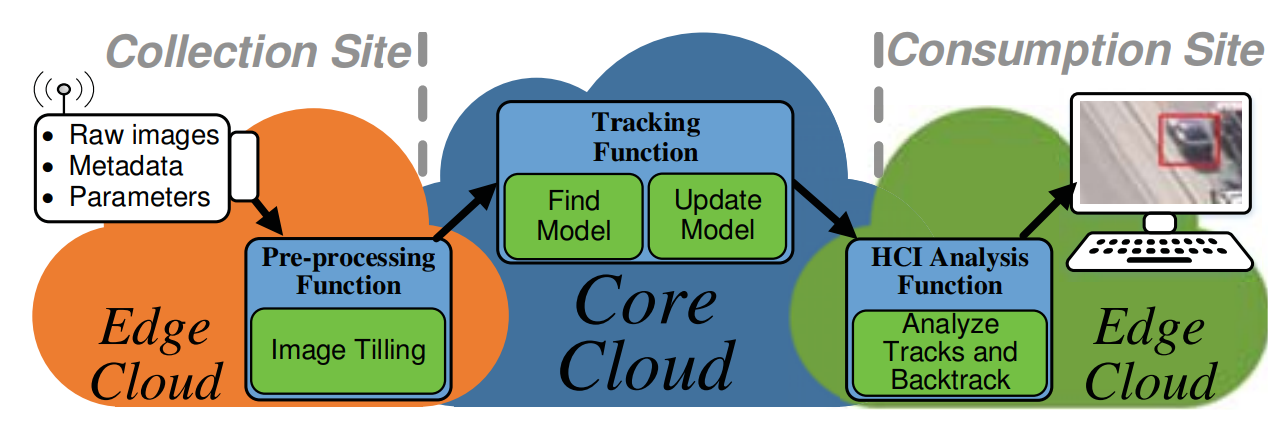
\includegraphics[width=0.8\textwidth]{figs/geosfc.PNG}
		\vspace{\baselineskip}
	\caption{Example 2: geo-distributed latency-sensitive SFC used
		for the real-time object tracking pipeline \cite{sfcgeo}}
	\label{fig:geosfc}
\end{figure}

%The majority of the existing works \cite{dynamicVNFedge, VNF5G, SFCedgecloud, Delay-awareVNFFlexibleResourceAllocation, PosterMEC, VNFmonoedgecore, LatencyAwareMEC} on SFC orchestration in MEC assume that system-wide information such as future service demand, user's mobility and network architecture is known, and one-shot solution is made based on this information, such problem is called \textit{system-managed placement}. However, in real MEC applications, the number of users and the diversity of their services and requirements limit the scalability and customizability of centralized system-managed solutions. \textit{online user-managed placement} is often considered due to user preference and system dynamics, In this model, each user is
%responsible for managing its own SFC with the help of the system that is provided through light-weight feedback.
%Recently, a few works have been proposed to use Reinforcement Learning (RL) based approaches to solve the online user-managed SFC placement~\cite{learningbasedvnf, QPlacement, Environment-AdaptiveRL, OnlineFault-tolerantDRL}. However, most of these works fail to address the SFC placement in a MEC context where features such as user's mobility and service migration are considered.
%Specifically, studies like \cite{MABserviceplacement} show that contextual user-managed algorithms are able to characterize mobile user behavior information and achieve better personalized support, in MEC system where system-level management is difficult due to the complexity of the edge cloud architecture.

The majority of previous research on SFC orchestration has focused on data center settings and does not consider edge resources and user mobility (\eg~\cite{minh_tnsm_20}). Thus, the existing works are not directly applicable to SFC orchestration in MEC. Those works that consider service orchestration in edge-enabled environments belong to one of the two classes: system-managed and user-managed methods. The system-managed methods orchestrate services from a centralized location (\eg~\cite{Spatio_temporal_TWC}). These works have an inherent uncertainty about the users' mobility and face scalability issues as the number of users increases. In contrast,  the user-managed methods enable end-users to manage their services in a distributed fashion based on the system feedback (\eg\ end-to-end delay). Several works use game theory to design user-managed mechanisms~\cite{8247219,8567670}. However, these works do not consider the migration cost and can not adapt to system changes. Recently, a few works have applied reinforcement learning and bandit formulation to provide a higher level of adaptability. In the face of problem complexity, these works have focused on the single VNF orchestration to limit the number of so-called \emph{arms} employed in the bandit formulation (\eg~\cite{MABserviceplacement}). We address this challenge by designing a user-managed SFC orchestration algorithm at the edge that applies reinforcement learning to minimize the user-perceived end-to-end delay while limiting the number of arms required for modeling SFCs by utilizing the theory of combinatorial bandits.


%
Therefore in this work, in order to take users' behavior into consideration while placing SFCs, we stand on the user-side perspective and propose an original contextual online learning approach that can cope with system uncertainty in edge and user-specific context.




\section{Thesis Objective}

In this thesis, we consider the problem of online SFC orchestration by mobile users with no prior knowledge of system side information (\ie, server capacities and link delays) in an edge-enabled environment, with the objective of minimizing the user-perceived end-to-end latency. More specifically, the uses generate a list of VNF demands representing the SFC request and decide which computing nodes they deploy the SFC on, yet they have no knowledge of the infrastructure information, including server capacities and link delays. The SFC orchestration is to decide, from the pool of resources available on the local device (\ie, hand-held equipment), at the edge and in a remote cloud, where to place each VNF of a service in order to minimize end-to-end service delay. In this optimization problem, there are three main difficulties that need to be considered:
\begin{itemize}
	\item \textit{Unknown environment}: The user has no knowledge of system information or future information.
	\item \textit{User's mobility}: User may roam throughout the MEC region during a continuous SFC-related service.
	\item \textit{VNF's migration}: VNF migration may be needed when the user moves too far from their original served region.
\end{itemize}



In our formulation of the problem, we consider the end-to-end service delay incurred due to processing, propagation, transmission, and service migration. We call this problem User-managed Edge-enabled Chain Orchestration Problem (\myproblem) and formulate it as a Mixed-Integer Program (MIP). To solve the problem, we design an algorithm, called \myalgorithm. In \myalgorithm, we employ the contextual combinatorial bandit framework to enable users to efficiently collect information from the environment and compute delay-optimized service placements. The context allows users to incorporate any available information (e.g., about demands) into the resource allocation formulation. We formulate the problem as a combinatorial bandit to focus on the basic user options (i.e., servers and links) during the learning phase of our algorithm, which significantly reduces the solution space of the problem. A naive formulation would force users to consider all possible solutions, whose number grows exponentially in terms of the number of servers and links (e.g., all the different paths in the network). 
Therefore, \myalgorithm\ can efficiently learn about the environment, i.e., fast convergence, without incurring a high processing penalty. For orchestrating services
efficiently, \myalgorithm\ uses a fast dynamic programming-based subroutine to make allocation and migration decisions based on the learned information. Finally, while the majority of exiting works in this area use numerical computations and simulations to evaluate their proposed algorithms, we use Mininet-WiFi to implement our proposed scheme and examine its performance and behavior in an emulated environment with a realistic setting and various mobility models.
%After the learning phase, the actual placement of services is done using a dynamic programming formulation that utilizes the learned information to compute a delay-optimized service placement



\section{Thesis Contribution}
In this section, we summarize the main contribution made by this work, including an overview of our proposed formulation and approach for \myproblem, and the experiments designed for evaluating the proposed approach.

\noindent\textbf{Customized Problem Formulation.}
We formulate the problem of user-managed SFC orchestration at the edge as an integer program by considering user demands, mobility, and end-to-end service delay, in which each formulation characterizes the key features in our work such as network models, delay models, and service models. The main constraints we consider in our formulation is designed to meet the network requirements, such as avoiding co-locating placement, single-path routing, and link bandwidth constraints. The objective of our problem is a weighted sum of four different delays we considered in our model. Specifically, we define multiple scale factors to specify the relative importance of different components of the end-to-end delay.

\noindent\textbf{Problem Transformation via Contextual CMAB.}
Due to the uncertainty of system-wide information and the visibility in the user-side state information, we are able to transform the user-managed SFC orchestration problem into a \textit{contextual combinatorial multi-arm bandit} problem. We formulate the delays in the network as arms that is to be selected and define various parameters to store information such as the unknown system feature and cumulative contextual feature.
The contextual combinatorial formulation allows the user to focus on the primitive options, thus greatly reduces the decision space and incorporate any available information to make better decisions. Furthermore, we adopted the \textit{contextual combinatorial upper confidence bound algorithm} (\ccucb) \cite{C^2MAB} in our decision making to balance exploration and exploitation. Lastly, We present a contextual combinatorial bandit learning algorithm to efficiently learn about the available resources on local equipment, at the edge, and in a remote cloud.

\noindent\textbf{Dynamic programming chain allocation.}
Our \ccmab\ formulation for user-managed SFC orchestration in MEC is an online learning problem that is unlikely to solve optimally due to the environment and time span uncertainty. However, at each learning slot, finding the current optimal SFC placement solution can be solved in a reasonable time with a traditional optimization method.
Therefore, we proposed a dynamic program (DP) based chain allocation method to optimally allocate SFC at each round, which takes the revealed estimates as input and take user-side specific contextual information into consideration. DP finds the optimal solution by starting from placing one single service and successively moving to the next service while taking the previous solutions into account. Our proposed DP-based approach is able to find the per-time-slot optimum in polynomial time.


% \noindent\textbf{Delay measurement framework.}
% A general CMAB framework assumes that, by selecting an arm, a certain estimation or outcome may be revealed. In order to satisfy this assumption, we proposed a time-stamp based delay measurement framework to obtain the delay experienced on a link or node of a SFC path. Moreover, we implement this framework in our Mininet-WiFi emulation.

\noindent\textbf{Simulation and Mininet-wifi emulation experiments.}
We present extensive simulation results to study the behavior of our algorithms under different experiment parameters and problem scales. 
By comparing to the offline optimum, we are able to show that our proposed approach can achieve a close-to-optimum performance.
We also compare the performance of our algorithms against two other greedy-based learning approaches and one offline benchmark to demonstrate the superior performance of the proposed algorithm. 
Furthermore, we simulate a MEC system with user mobility using \textit{mininet-wifi} \cite{mininetwifi} and implement manageable VNFs for each server node.
We then perform a set of experiments in Mininet-WiFi to validate the practical performance of the proposed algorithm.



\section{Thesis Organization.}
The thesis is divided into nine chapters. The content of each chapter is summarized below.

\dog{Chapter 1} discussed the motivation for this study, provides a summary of the current research scope and our research objective, as well as an outline of the main contributions in this work.

\dog{Chapter 2}  provides the necessary background on NFV, MEC, SFC techniques, discusses the online learning approaches as well as the mathematical optimization techniques employed in this study, and gives an overview of the software tools used in experiments.

\dog{Chapter 3} reviews the most relevant literature that focuses on SFC placement problems and classifies them into different categories based on whether they are edge-enabled and user-managed.

\dog{Chapter 4} describes the system model and present the optimization formulation for offline \myproblem.

\dog{Chapter 5} presents the contextual combinatorial bandit formulation for the proposed SFC placement problem and the design of our proposed dynamic programming-based online learning algorithm.

\dog{Chapter 6} presents the design of a time-stamp based delay estimation method that is required in the bandit formulation.

\dog{Chapter 7} presents the extensive simulations results to study the learning behavior of the proposed algorithms and demonstrate their superior performance on scalability compared to the greedy approaches. 

\dog{Chapter 8} presents the Mininet-WiFi experiment results to validate the practical performance of the proposed approach 

\dog{Chapter 9} concludes the thesis with a summary of the works and discussions for future research orientations.








